\documentclass[11pt,usenames,dvipsnames,
  hyperref={pdfencoding=auto,psdextra}]{beamer}
\usepackage{gensymb}

\newcommand*{\listsofb}[1]{\mathcal{L} (#1)}
\newcommand*{\listsof}{\mathcal{L}~}

\newcommand{\None}{\emptyset}
\newcommand{\Some}[1]{\degree\kern-0.5ex#1}
\newcommand{\lnil}{\ensuremath{[]}}

\newcommand*{\match}{\textbf{match}~}
\newcommand*{\withl}{\textbf{[}~}
\newcommand*{\withr}{~\textbf{]}}
\newcommand*{\withm}{\quad\textbf{|}\quad}
\newcommand*{\llet}{\textbf{let}~}
\newcommand*{\lin}{\textbf{in}~}
\newcommand{\ITE}[3]{\textbf{if}~{#1}~\textbf{then}~{#2}~\textbf{else}~{#3}}

\newcommand{\Type}{\mathbb{T}}
\newcommand{\Prop}{\mathbb{P}}
\newcommand{\bool}{\mathbb{B}}
\newcommand{\btrue}{\mathsf{T}}
\newcommand{\bfalse}{\mathsf{F}}
\newcommand{\andb}{\&\&}
\newcommand{\orb}{||}
\newcommand{\notb}{!}
\newcommand{\nat}{\mathbb{N}}
\newcommand{\natS}{1 + }
\newcommand{\length}[1]{|#1|}

\newcommand{\con}{\mathop{{+}\!\!\!{+}}}
\newcommand{\rev}{\mathsf{rev}}
\newcommand{\opt}[1]{\mathcal{O}{#1}}

\newcommand{\eqb}[2]{#1\overset{?}{=}#2}

\usepackage[english]{babel}
\usepackage{lipsum}
\usepackage{pifont}
\usepackage{booktabs}
\usepackage{multirow}
\usepackage[absolute,overlay]{textpos}
\usepackage{proof}
\usepackage{amsmath}
%\usepackage[utf8]{inputenc}
\usepackage{listings}
\usepackage{tikz}
\usetikzlibrary{automata,trees,calc,arrows.meta,positioning,decorations.pathreplacing,bending,shapes.geometric, intersections, hobby}
\usetheme{Berlin}
\usepackage{cite}
\usepackage{cancel}
\usepackage{xsavebox}
\usepackage[normalem]{ulem}
\usepackage{array}
\usepackage{wasysym}
\usepackage{pgfplots}


\pgfplotsset{compat=1.16}

%some nicer colour scheme
\definecolor{craneorange}{RGB}{237, 142, 26}
\definecolor{craneblue}{RGB}{0,0,0}

\setbeamercolor{structure}{fg=craneblue}

\setbeamercolor{palette primary}{fg=craneblue,bg=craneorange!70}
\setbeamercolor{palette secondary}{fg=craneblue,bg=craneorange!80}
\setbeamercolor{palette tertiary}{fg=craneblue,bg=craneorange!90}
\setbeamercolor{palette quaternary}{fg=craneblue,bg=craneorange}

\setbeamercolor{titlelike}{parent=palette quaternary}

\setbeamercolor{block title}{fg=craneblue,bg=craneorange}
\setbeamercolor{block title alerted}{use=alerted text,fg=craneblue,bg=alerted text.fg!75!bg}
\setbeamercolor{block title example}{use=example text,fg=craneblue,bg=example text.fg!75!bg}

\setbeamercolor{block body}{parent=normal text,use=block title,bg=block title.bg!15!bg}
\setbeamercolor{block body alerted}{parent=normal text,use=block title alerted,bg=block title alerted.bg!15!bg}
\setbeamercolor{block body example}{parent=normal text,use=block title example,bg=block title example.bg!15!bg}

\setbeamercolor{sidebar}{bg=craneorange!70}

\setbeamercolor{palette sidebar primary}{fg=craneblue}
\setbeamercolor{palette sidebar secondary}{fg=craneblue!75}
\setbeamercolor{palette sidebar tertiary}{fg=craneblue!75}
\setbeamercolor{palette sidebar quaternary}{fg=craneblue}

\setbeamercolor*{separation line}{}
\setbeamercolor*{fine separation line}{}

\setbeamercolor{frametitle}{bg=white}

%no frame numbering when using framebreaks
\setbeamertemplate{frametitle continuation}{}

%no total frame number
\setbeamertemplate{footline}{% 
  \hfill% 
  \usebeamercolor[fg]{page number in head/foot}% 
  \usebeamerfont{page number in head/foot}% 
  \insertframenumber%
  %\,/\,\inserttotalframenumber
  \kern1em\vskip2pt% 
}

%no subsection line
\setbeamertemplate{headline}
{%
  \begin{beamercolorbox}[colsep=1.5pt]{upper separation line head}
  \end{beamercolorbox}
  \begin{beamercolorbox}{section in head/foot}
    \vskip0pt\insertnavigation{\paperwidth}\vskip3pt
  \end{beamercolorbox}%
  \begin{beamercolorbox}[colsep=1.5pt]{lower separation line head}
  \end{beamercolorbox}
}

%highlight colours to be used throughout the presentation
\newcommand{\highlight}[1]{\color{blue}#1\color{black}}
\newcommand{\colorHOne}{\color{red}}
\newcommand{\colorHThree}{\color{violet}}
\newcommand{\colorHTwo}{\color{blue}}

\newcommand{\colorTikzA}{red}
\newcommand{\colorTikzB}{cyan}
\newcommand{\colorTikzC}{blue}
\newcommand{\colorTikzD}{green}

%don't count the title page
\let\otp\titlepage
\renewcommand{\titlepage}{\otp\addtocounter{framenumber}{-1}}

%a hide on=... option for tikz elements, where the usual ranges allowed by \only are allowed for ...
\tikzset{hide on/.code={\only<#1>{\pgfkeysalso{white}}}}

%don't want those nasty navigation symbols
\beamertemplatenavigationsymbolsempty


\newenvironment{tightcenter}{%
  \setlength\topsep{0pt}
  \setlength\parskip{0pt}
  \begin{center}
    }{%
  \end{center}
}

%table column types for fixed width
\newcolumntype{L}[1]{>{\raggedright\let\newline\\\arraybackslash\hspace{0pt}}m{#1}}
\newcolumntype{C}[1]{>{\centering\let\newline\\\arraybackslash\hspace{0pt}}m{#1}}
\newcolumntype{R}[1]{>{\raggedleft\let\newline\\\arraybackslash\hspace{0pt}}m{#1}}

%TODO
\newcommand\TODO{
  \colorbox{red}{TODO}
}

%math stuff
\newcommand*{\Eq}{\text{Eq}}
\newcommand*{\N}{\mathbb{N}}
\newcommand*{\R}{\mathbb{R}}
\newcommand*{\Reach}{\text{Reach}}
\newcommand*{\norm}[1]{\left\lVert#1\right\rVert}
\newcommand*{\diff}{\text{d}}
\newcount\colveccount
\newcommand*\colvec[1]{
        \global\colveccount#1
        \begin{pmatrix}
        \colvecnext
}
\def\colvecnext#1{
        #1
        \global\advance\colveccount-1
        \ifnum\colveccount>0
                \\
                \expandafter\colvecnext
        \else
                \end{pmatrix}
        \fi
}


%prevent backup slides from appearing in the header
\makeatletter
\let\beamer@writeslidentry@miniframeson=\beamer@writeslidentry%
\def\beamer@writeslidentry@miniframesoff{%
  \expandafter\beamer@ifempty\expandafter{\beamer@framestartpage}{}% does not happen normally
  {%else
    % removed \addtocontents commands
    \clearpage\beamer@notesactions%
  }
}
\newcommand*{\miniframeson}{\let\beamer@writeslidentry=\beamer@writeslidentry@miniframeson}
\newcommand*{\miniframesoff}{\let\beamer@writeslidentry=\beamer@writeslidentry@miniframesoff}
\makeatother


%footnote without marker, for images
\newcommand\blfootnote[1]{%
  \begingroup
  \renewcommand\thefootnote{}\footnote{#1}%
  \addtocounter{footnote}{-1}%
  \endgroup
}

\newcommand{\bnfmid}{~\mid~}


\title{A Formal Study of Complexity Theory Using the Call-by-Value $\lambda$-Calculus in Coq}

\institute{Saarland University}
\date{8 November 2019}
\author{Lennard Gäher\\[1mm] {\small{Advisor: Fabian Kunze}}}

\begin{document}
\begin{frame}[plain]
  \titlepage
\end{frame}

\section{Introduction}
\begin{frame}{Timeline}
  \begin{tikzpicture}[overlay,remember picture]
    \node[minimum width=\paperwidth,minimum height =\paperheight,anchor=north west] (a) {};
    \draw[thick,->] ($(current page.north east)!0.5!(current page.north west) + (0, -0.57)$) -- ($(current page.south west)!0.5!(current page.south east) + (0, 1)$);
  \end{tikzpicture}

  \setlength{\TPHorizModule}{\textwidth}
  \setlength{\TPVertModule}{\textwidth}
  \begin{textblock}{0.5} (0.62, 0.2)
    \small
    \textbf{1964:} DTIME, time hierarchy,\ldots

    \emph{Computational complexity of recursive sequences}

    Hartmanis and Stearns
  \end{textblock}

    \begin{textblock}{0.5} (0.05, 0.5)
      \onslide<2->{
        \small 
        \textbf{1971:} Cook's Theorem

        \emph{The Complexity of Theorem-Proving Procedures}

        Stephen A.\ Cook
      }
    \end{textblock}

    \begin{textblock}{0.5} (0.62, 0.6)
    \onslide<3->{
        \small
        \textbf{1972:} Karp's 21 NP-complete problems

        \emph{Reducibility Among Combinatorial Problems}

        Richard M.\ Karp
      }
    \end{textblock}
\end{frame}

\newcommand{\Term}{\textsf{Term}}

\begin{frame}{The Call-by-Value $\lambda$-calculus L\footnote{\cite{ForsterSmolka:2017:L-Computability}} \ldots}
  \begin{align*}
    s, t : \Term := n \bnfmid s~t \bnfmid \lambda s
  \end{align*}

  \begin{align*}
    \infer{(\lambda s)(\lambda t) \succ s^0_{\lambda t}}{}
    && 
    \infer{s~t \succ s'~t}{s \succ s'}
    && 
    \infer{s~t \succ s~t'}{t \succ t'}
  \end{align*}
  \begin{alignat*}{2}
    &k^k_u := u \qquad& n^k_u := n \qquad \mathit{if}~n\neq k \\
    & {(s~t)}^k_u := (s^k_u)~(t^k_u) 
    \qquad & {(\lambda s)}^k_u := \lambda(s^{\natS k}_u)
  \end{alignat*}
\end{frame}


\begin{frame}{\ldots as a Model of Computation}
  \begin{block}{Scott Encoding (of Numbers)}
    \vspace{-1ex}
    \begin{align*} 
      \overline{0} = \lambda\lambda. 1\\
      \overline{S~n} = \lambda\lambda. 0~(\overline n)
    \end{align*}
    \vspace{-1ex}
  \end{block}
  %similarly for other inductive types. mention encoding/decoding
\end{frame}
\begin{frame}[noframenumbering]{\ldots as a Model of Computation}

  \begin{itemize}
    \item certifying extraction from Coq to L\footnote{\cite{ForsterKunze:2019:Certifying-extraction}}, including time bounds
      \begin{itemize}
        \item inductive datatypes
        \item recursive functions
      \end{itemize}
    \item<2-> reasonable for time and space\footnote{\cite{ForsterKunzeRoth:2019:wcbv-Reasonable}}
      \begin{gather*}
        \textsf{size}~n := 1 \\
        \textsf{size}~(s~t) := \textsf{size}~s + \textsf{size}~t + 1 \\ 
        \textsf{size}~(\lambda s) := \textsf{size}~s + 1
      \end{gather*}
  \end{itemize}

\end{frame}

\begin{frame}{Basic Definitions: NP}
  Language $A : X \rightarrow \Prop$

  \vspace{2ex}
  $\textsf{inNP}~A$, if:
  \begin{itemize}
    \item there is a verifier $V : X \rightarrow \Term \rightarrow \Prop$
    \item $\forall x, A~x \leftrightarrow \exists~\mathit{cert}, V~x~\mathit{cert}$
    \item $V$ is polynomial-time computable (in $\textsf{size}(\overline x), \textsf{size}(\overline{cert})$)
    \item $\exists p, \forall x y, V~x~y \rightarrow \textsf{size}(\overline y) \le p(\textsf{size}(\overline x))$
  \end{itemize}
  \vspace{2ex}
  $p,q$: monotonic and polynomially bounded
\end{frame}

\begin{frame}{Basic Definitions: Polynomial-time Reductions}
  \[A : X \rightarrow \Prop \qquad B : Y \rightarrow \Prop\]

  \begin{align*}
    A \preceq_{\text{p}} B := \exists f : X \rightarrow Y, \quad&(\forall x, A~x \leftrightarrow B(f~x)) \\
    \land& \text{ polynomial-time computable } f\\
    \land &\exists~p, \forall x, \textsf{size}{(\overline{f~x})} \le p(\textsf{size}{(\overline{x})}) 
  \end{align*}
  
  \begin{align*}
    \textsf{NP-hard}~A := \forall B, \textsf{inNP}~B \rightarrow B \preceq_{\text{p}} A 
  \end{align*}
\end{frame}

\section{3-SAT $\prec_\text{p}$ Clique}
\newcommand{\var}{\textsf{var}}
\newcommand{\literal}{\textsf{literal}}
\newcommand{\clause}{\textsf{clause}}
\newcommand{\cnf}{\textsf{cnf}}
\newcommand{\assgn}{\textsf{assgn}}

\newcommand*{\eval}[2]{\mathcal{E}~#1~#2~}

\begin{frame}{SAT}
  \begin{alignat*}{14}
    (&x_0& \lor &\overline{x_1}& \lor &x_2&) &\land &(&x_0& \lor &x_3 &\lor &x_1&)\\
    \only<1-2>{&&&\color{white}\overline{\btrue}&&&&&&&&&&} %in order to prevent shifting
    \only<3>{\color{gray} (&\color{gray}\btrue&\color{gray} \lor &\color{gray}\overline{\bfalse} &\color{gray}\lor &\color{gray}\bfalse&\color{gray}) &\color{gray}\land& \color{gray}(&\color{gray}\btrue&\color{gray} \lor &\color{gray}\bfalse &\color{gray}\lor &\color{gray}\bfalse&\color{gray}) }
    \only<4>{\color{gray} &\color{white}\overline{\btrue} &&\color{gray} \btrue & & && \color{gray}\land && & & \color{gray}\btrue & & & }
    \only<5>{ & \color{white}{\overline{\btrue}}&& &&&& \color{gray} \btrue &&&&\color{white} \btrue&&&}
  \end{alignat*}
  \vspace{-2ex}
  \onslide<2->
  \[\{x_0 \mapsto \btrue, x_1 \mapsto \bfalse, x_2 \mapsto \bfalse, x_3 \mapsto \bfalse\}\]

  \onslide<5->
  \[\text{Evaluation}~ \mathcal{E} : \assgn \rightarrow \cnf \rightarrow \opt{(\bool)} \]

  \onslide<5->
  \begin{definition}[SAT]
    \[\textbf{SAT}~N := \exists~a, \eval{a}{N}~=~\Some{\btrue} \]
  \end{definition}

\end{frame}


\begin{frame}{SAT}
  \begin{definition}[$k$-SAT]
    \begin{align*}
      \infer{\textsf{$k$-CNF}~[]}{} && \infer{\textsf{$k$-CNF}~(C::N)}{\textsf{$k$-CNF}~N \quad \length{C} = k} 
    \end{align*}
    \[\textbf{$k$-SAT}~N := \textsf{$k$-CNF}~N \land \exists~a, \eval{a}{N} ~=~\Some{\btrue} \]
  \end{definition}
\end{frame}

\newcommand{\lnode}{\textsf{node}}
\newcommand{\ledge}{\textsf{edge}}
\newcommand{\lgraph}{\textsf{graph}}

\begin{frame}{Clique}
  \begin{center}
  \begin{tikzpicture} [shorten >=1pt,node distance=2cm,on grid, auto, baseline] 
    \node[state] (S_0)   {}; 
    \node[state] (S_1) [right=of S_0] {}; 
    \node[state] (S_2) [below=of S_0] {}; 
    \node[state] (S_3) [right=of S_2] {};
    \only<1,4>{\path (S_0) edge (S_1);}
    \path (S_0) edge (S_3);
    \only<1,2,4>{\path (S_0) edge (S_2);}
    \only<1,2,4>{\path (S_1) edge (S_2);}

    \path (S_2) edge (S_3);

    \only<2,3>{\path (S_0) edge[thick,color=\colorTikzA] (S_1);}
    \only<3>{\path (S_0) edge[thick,color=\colorTikzA] (S_2);}
    \only<3>{\path (S_1) edge[thick, color=\colorTikzA] (S_2);}

      \only<4>{\path (S_1) edge[color=\colorTikzC] (S_3);}
    \end{tikzpicture}
  \end{center}


%\begin{align*}
  %u,v : \lnode := \nat \\
  %e : \ledge := \lnode \times \lnode &&\textit{-- undirected!}\\
  %g : \lgraph := \nat \times \listsof~\ledge 
%\end{align*}

\end{frame}

\begin{frame}[allowframebreaks]{Clique}
  \begin{columns}
\begin{column}{0.48\textwidth}
  \begin{center}
  \begin{tikzpicture} [shorten >=1pt,on grid, auto, baseline,scale=0.5,every node/.style={scale=0.5}] 
    \node[state] (S_0)   {}; 
    \node[state] (S_1) [right=of S_0] {}; 
    \node[state] (S_2) [below=of S_0] {}; 
    \node[state] (S_3) [right=of S_2] {};
    \only<1,4>{\path (S_0) edge (S_1);}
    \path (S_0) edge (S_3);
    \only<1,2,4>{\path (S_0) edge (S_2);}
    \only<1,2,4>{\path (S_1) edge (S_2);}

    \path (S_2) edge (S_3);

    \only<2,3>{\path (S_0) edge[thick,color=\colorTikzA] (S_1);}
    \only<3>{\path (S_0) edge[thick,color=\colorTikzA] (S_2);}
    \only<3>{\path (S_1) edge[thick, color=\colorTikzA] (S_2);}

      \only<4>{\path (S_1) edge[color=\colorTikzC] (S_3);}
    \end{tikzpicture}
  \end{center}
\end{column}

\begin{column}{0.48\textwidth}
\begin{align*}
  u,v : \lnode \\
  e : \ledge \\
  g : \lgraph 
\end{align*}
\end{column}
\end{columns}

\begin{definition}[$k$-Clique]
  \begin{gather*}
    \infer{\textsf{isClique}~g~[]~0}{}\\[1.2ex]
    \infer{\textsf{isClique}~g~(v::cl)~(\natS{k})}{v \notin cl \quad \textsf{nodeIn}~g~v \quad (\forall u \in cl, \textsf{edgeIn}~g~v~u) \quad \textsf{isClique}~g~cl~k}
  \end{gather*}
\end{definition}

\begin{definition}[Clique]
  %TODO: maybe add well-formedness
  \[\textbf{Clique}~(g, k) := \exists~cl, \textsf{isClique}~g~cl~k\]
\end{definition}
\end{frame}

\newcommand*{\redrel}{\ensuremath{\sim^{\text{3-\textbf{SAT}}}_{\textbf{Clique}}}}

\begin{frame}[noframenumbering]
\[\scalebox{1.5}{$3-\textbf{SAT} \prec_{\text{p}} \textbf{Clique}$}\]
\end{frame}


\begin{frame}{Reduction: Example}
  \begin{columns}
    \begin{column}{0.44\textwidth}
  $(x_0 \lor \overline{x_1} \lor x_2) \land (x_0 \lor x_3 \lor x_1)$
\end{column}
\begin{column}{0.52 \textwidth}
  \raggedleft
  %\only<6>{\colorHOne{} $\overline{x_1}, x_3$}
  %\only<7>{\colorHOne{} $[F, F, T, F]$}
\end{column}
\end{columns}
  \vspace{4ex}

  \begin{center}
\begin{tikzpicture}[node distance=2.2cm, shorten >=1pt,on grid, auto, baseline] 
  \node[state, label={[]180:$x_0$}] (00) {\only<1>{\color{white}}{\small(0, 0)}};
  \node[state,below=of 00, label={[]180:$\overline{x_1}$}] (01) {\only<1>{\color{white}}{\small(0, 1)}};
  \node[state,below=of 01, label={[]180:$x_2$}] (02) {\only<1>{\color{white}}{\small(0, 2)}};
  \node[state,right =3cm of 00, label={[]0:$x_0$}] (10) {\only<1>{\color{white}}{\small(1, 0)}};
  \node[state,below=of 10, label={[]0:$x_3$}] (11) {\only<1>{\color{white}}{\small(1, 1)}};
  \node[state,below=of 11, label={[]0:$x_1$}] (12) {\only<1>{\color{white}}{\small(1, 2)}};

  \only<3-> {
    \path (00) edge (10)
      (00) edge (11)
      (00) edge (12);
  }

  \only<4-> {
    \path (01) edge (10);
  }
  \only<4-5>{
      \path (01) edge (11);
  }

  \only<5-> {
    \path (02) edge (10)
      (02) edge (11)
      (02) edge (12);
  }

  %\only<6-> {
    %\path (01) edge[color=\colorTikzA, thick] (11);
  %}
\end{tikzpicture}
\end{center}
\only<2>{}

\end{frame}

\begin{frame}{Reduction Relation}
  \begin{gather*}
    \only<1>{N \overset{f}{\mapsto} (g, \length{N})} 
    \only<2->{N \redrel (f~N)}\\[3ex]
    \only<2->{N \redrel (g, \length{N}) \rightarrow} \text{3-\textbf{SAT}}~N \leftrightarrow \textbf{Clique}~(g, \length{N})
  \end{gather*}

  \onslide<3->{
    \begin{center}
      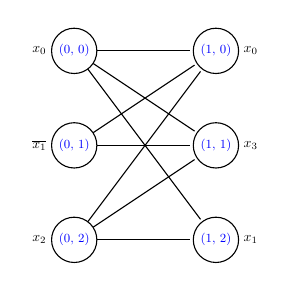
\begin{tikzpicture}[node distance=1.2cm, shorten >=1pt,on grid, auto, baseline, scale=0.5,every node/.style={scale=0.5}] 
        \node[state, label={[]180:$x_0$}] (00) {{\colorHTwo\small(0, 0)}};
        \node[state,below=of 00, label={[]180:$\overline{x_1}$}] (01) {{\colorHTwo\small(0, 1)}};
        \node[state,below=of 01, label={[]180:$x_2$}] (02) {{\colorHTwo\small(0, 2)}};
        \node[state,right =1.8cm of 00, label={[]0:$x_0$}] (10) {{\colorHTwo\small(1, 0)}};
        \node[state,below=of 10, label={[]0:$x_3$}] (11) {{\colorHTwo\small(1, 1)}};
        \node[state,below=of 11, label={[]0:$x_1$}] (12) {{\colorHTwo\small(1, 2)}};

        \path (00) edge (10)
          (00) edge (11)
          (00) edge (12);

        \path (01) edge (10);

        \path (01) edge (11);

        \path (02) edge (10)
          (02) edge (11)
          (02) edge (12);
      \end{tikzpicture}
    \end{center}
  }

\end{frame}

\begin{frame}[t]{Correctness}
  {$\scalebox{1.2}{$N \redrel{} (g, \length{N})$}$}
  \vspace{-4ex}
  \only<1>{\[ \text{3-\textbf{SAT}}~N \leftrightarrow \textbf{Clique}~(g, \length{N}) \]}
  \only<2->{\[(\exists~a, \eval{a}{N} = \Some{\btrue}) \only<2>{\leftrightarrow} \only<3->{\rightarrow} (\exists~cl, \textsf{isClique}~g~cl~k)\]}

  \onslide<3->
  \begin{itemize}
    \item Pick a satisfied literal for each clause
    \item A clique is given by the the corresponding nodes
  \end{itemize}
\end{frame}

\begin{frame}[t]{Correctness}
  {$\scalebox{1.2}{$N \redrel (g, k)$}$}
  \vspace{-4ex}
  \[(\exists~a, \eval{a}{N} = \Some{\btrue}) \leftarrow (\exists~cl, \textsf{isClique}~g~cl~(\length{N}))\]

  \begin{enumerate}
    \item<3-> Map clique nodes to literal positions
    \item<4-> Map literal positions to syntax of literals
    \item<5-> Expand to full assignment
  \end{enumerate}

    \vspace{-1.5ex}
  \begin{overlayarea}{\textwidth}{0.35\textwidth}
    \begin{columns}
      \begin{column}{0.48 \textwidth}
        \newcommand*{\highlightcolor}{black}
        \only<2-3>{\renewcommand*\highlightcolor{\colorTikzA}}

        \begin{center}
          \vspace{-6ex}
          \[(x_0 \lor \overline{x_1} \lor x_2) \land (x_0 \lor x_3 \lor x_1)\]
          \begin{tikzpicture}[node distance=1.2cm, shorten >=1pt,on grid, auto, baseline, scale=0.5,every node/.style={scale=0.5}] 
            \node[state, label={[]180:$x_0$}] (00) {{\small(0, 0)}};
            \node[state,below=of 00, label={[]180:$\overline{x_1}$},draw=\highlightcolor] (01) {{\small(0, 1)}};
            \node[state,below=of 01, label={[]180:$x_2$}] (02) {{\small(0, 2)}};
            \node[state,right =1.8cm of 00, label={[]0:$x_0$}] (10) {{\small(1, 0)}};
            \node[state,below=of 10, label={[]0:$x_3$},draw=\highlightcolor] (11) {{\small(1, 1)}};
            \node[state,below=of 11, label={[]0:$x_1$}] (12) {{\small(1, 2)}};

              \path (00) edge (10)
                (00) edge (11)
                (00) edge (12);

              \path (01) edge (10);

            \only<1,4->{
                \path (01) edge (11);
              }

              \path (02) edge (10)
                (02) edge (11)
                (02) edge (12);

            \only<2-3> {
              \path (01) edge[color=\colorTikzA, thick] (11);
            }
          \end{tikzpicture}
        \end{center}
      \end{column}
      \begin{column}{0.48 \textwidth}
        \begin{align*}
          \only<-2>{\color{white}}\rightarrow \quad& \only<-2>{\color{white}} [(0, 1), (1, 1)] \\[3.3ex]
          \only<-3>{\color{white}} \rightarrow \quad& \only<-3>{\color{white}} [\overline{x_1}, x_3] \\[3.3ex]
          \only<-4> {\color{white}} \rightarrow \quad& \only<-4>{\color{white}} \{x_0 \mapsto {\only<5->{\color{gray}}\bfalse,} x_1 \mapsto {\bfalse}, {\only<5->{\color{gray}} x_2 \mapsto \bfalse,} x_3 \mapsto {\btrue}\}
        \end{align*}
      \end{column}
    \end{columns}
  \end{overlayarea}
\end{frame}

\begin{frame}{Reduction Function}
  \[f : \cnf \rightarrow \textsf{graph} \times \nat \text{ with } N \redrel (f~N) \]
\end{frame}

\begin{frame}[t]{Time Analysis: Example}
  \vspace{-5ex}
  \begin{align*}
    \text{Show: polynomial-time computable } f
  \end{align*}

  \begin{align*}
    \textsf{forallb}~&: (A \rightarrow \bool) \rightarrow \listsof{A} \rightarrow \bool\\
    \textsf{forallb}~&f~\lnil := \btrue \\
    \textsf{forallb}~&f~(l::ls) := f~a~\andb~\textsf{forallb}~f~ls
  \end{align*}

  \onslide<2->
  \begin{align*}
    \textsf{forallb\_time}~(fT : A \rightarrow \nat)~l := \textsf{foldr}~(\lambda~el~acc.~fT~el + acc + 15)~8~l 
  \end{align*}

  \begin{overlayarea}{\textwidth}{0.3\textwidth}
    \only<3>{
    \begin{align*}
      \forall~&(fT: A \rightarrow \nat), \\
        &(\exists~(p : \nat \rightarrow \nat), \forall~el, fT~el \le p(\textsf{size}(\overline{el}))) \\
        \rightarrow &~\exists ~(p : \nat \rightarrow \nat), \forall~l, \textsf{forallb\_time}~fT~\le p(\textsf{size}(\overline{l}))
    \end{align*}
  }

    \only<4>{
    \begin{align*}
      \forall~&(fT: {\colorHOne E \rightarrow} A \rightarrow \nat), \\
              &(\exists~(p : \nat \rightarrow \nat), \forall~el~{\colorHOne env}, fT~{\colorHOne env}~el \le p(\textsf{size}(\overline{el}) {\colorHOne + \textsf{size}(\overline{env})})) \\
              \rightarrow &~\exists ~(p : \nat \rightarrow \nat), \forall~l~{\colorHOne env}, \textsf{forallb\_time}~{\colorHOne (fT~env)}~l\le p(\textsf{size}(\overline{l}) {\colorHOne + \textsf{size}(\overline{env})})
    \end{align*}
  }
  \end{overlayarea}
\end{frame}

\begin{frame}<1-3>[label=abstractions]{Problem: Abstractions}
  \frametitle<4>{Problem: Abstractions, Revisited}
  \begin{itemize}
    \item explicit construction and analysis of reduction function 
      \begin{itemize}
        \item no implicit proof mode constructions
        \item little potential for automation
      \end{itemize}
    \item<2-> simple representations due to extraction and time analysis
      \begin{align*}
        u,v : \lnode := \nat \\
        e : \ledge := \lnode \times \lnode\\
        g : \lgraph := \nat \times \listsof~\ledge 
      \end{align*}
    \item<3-> {\only<4>{\colorHOne} {``global'' structure as in \textbf{Clique}}}
  \end{itemize}
\end{frame}

\section{Towards Cook's Theorem}
\begin{frame}{Cook's Theorem}
  \begin{block}{\vspace*{-3ex}}
    \textbf{SAT} is NP-hard.
  \end{block}
  %outline: we reduce from Turing machines instead of L because of the simpler (low-level) structure
  %need reduction from L to TM in order to derive NP-hardness - TODO: Fabian is currently working on that

  \vspace{5ex}

  \onslide<2->
  \begin{block}{Generic Problem}
    \begin{overlayarea}{\textwidth}{0.1\textwidth}
      \only<2>{
        $\textbf{GenNP}~(M, \mathit{input}, t) := M$ is a nondet.\ TM $\land M$ accepts on $\mathit{input}$ in $\le t$ steps    
      }
      \only<3->{
        $\textbf{GenNP}~(M, k, t) := M$ is a det.\ TM $\land \exists~\mathit{input}, \length{input} \le k \land$ $M$ accepts on $\mathit{input}$ in $\le t$ steps
      }
  \end{overlayarea}
  \end{block}
\end{frame}

\begin{frame}{}
  \begin{tikzpicture}[overlay, remember picture]
    \draw (1.5, -4) -- (1.5, 3) -- (8.5, 3) -- (8.5, -4) -- (1.5, -4);
    \draw (2, -4) -- (2, 3);
    \draw (8, -4) -- (8, 3);
    \draw (1.5, 2.5) -- (8.5, 2.5);
    \draw (1.5, -3.5) -- (8.5, -3.5);
    \draw (1.5, 2) -- (8.5, 2);
    \draw (1.5, 1.5) -- (2, 1.5);
    \draw (8, 1.5) -- (8.5, 1.5);

    \draw (2.5, 3) -- (2.5, 2);
    \draw (3, 3) -- (3, 2.5);
    \draw (4.5, 3) -- (4.5, 2.5);
    \draw (5, 3) -- (5, 2.5);
    \draw (5.5, 3) -- (5.5, 2.5);
    \draw (7.5, 3) -- (7.5, 2.5);

    \node at (1.75, 2.75) {\small \#};
    \node at (1.75, 2.25) {\small \#};
    \node at (1.75, 1.75) {\small \#};
    \node at (1.75, -3.75) {\small \#};
    \node at (8.25, 2.75) {\small \#};
    \node at (8.25, 2.25) {\small \#};
    \node at (8.25, 1.75) {\small \#};
    \node at (8.25, -3.75) {\small\#};

    \node at (2.25, 2.75) {$q_0$};
    \node at (5.25, 2.75) {\textvisiblespace};
    \node at (7.75, 2.75) {\textvisiblespace};
    \node at (3.75, 2.75) {$\ldots$};
    \node at (6.5, 2.75) {$\ldots$};
    \node at (5, 2.25) {$\ldots$};
    \node at (1.75, -0.375) {$\vdots$};
    \node at (8.25, -0.375) {$\vdots$};

    \draw (4, -0.5) -- (4, 0.5) -- (5.5, 0.5) -- (5.5, -0.5) -- (4, -0.5);
    \draw (4.5, -0.5) -- (4.5, 0.5);
    \draw (5, -0.5) -- (5, 0.5);
    \draw (4, 0) -- (5.5, 0);

    \path[<->] (1, -4) edge node[fill=white, anchor=center, pos= 0.5] {\small t} (1, 3);
    \path[<->] (1.5, -4.5) edge node[fill=white, anchor=center, pos=0.5] {\small t} (8.5, -4.5);
    \path[<->] (2.5, 3.5) edge node[fill=white, anchor=center, pos=0.5] {\small k} (5, 3.5);

    \node at (9.5, 2.75) {\small 1\textsuperscript{st} config};
    \node at (9.5, 2.25) {\small 2\textsuperscript{nd} config};
    \node at (9.5, 1.75) {\small 3\textsuperscript{rd} config};
  \end{tikzpicture}
\end{frame}

\newcommand{\cmark}{\ding{51}}
\newcommand{\xmark}{\ding{55}}

\begin{frame}
  \[\delta(q_1, a) = (q_1, b, R), \delta(q_1, b) = (q_2,c, L) \]

  \begin{columns}
    \begin{column}{0.3\textwidth}
      \begin{center}
        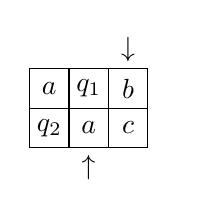
\begin{tikzpicture}
          \draw (0, 0) -- (0, 1) -- (1.5, 1) -- (1.5, 0) -- (0, 0);
          \draw (0.5, 0) -- (0.5, 1);
          \draw (1, 0) -- (1, 1);
          \draw (0, 0.5) -- (1.5, 0.5);

          \node at (0.25, 0.25) {$ q_2$};
          \node at (0.75, 0.25) {$ a$};
          \node at (1.25, 0.25) {$c$};

          \node at (0.25, 0.75) {$a$};
          \node at (0.75,  0.75) {$q_1$};
          \node at (1.25, 0.75) {$b$};

          \onslide<2->{
            \node at (1.25, 1.25) {$\downarrow$};
            \node at (0.75, -0.25) {$\uparrow$};

          }
          \onslide<3->{
            \node at (2, 0.5) {\cmark};
          }
        \end{tikzpicture}
      \end{center}
    \end{column}
    \begin{column}{0.3\textwidth}
      \begin{center}
        \onslide<4->{
          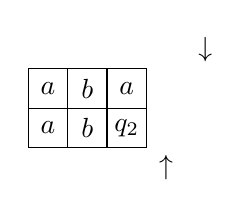
\begin{tikzpicture}
            \draw (0, 0) -- (0, 1) -- (1.5, 1) -- (1.5, 0) -- (0, 0);
            \draw (0.5, 0) -- (0.5, 1);
            \draw (1, 0) -- (1, 1);
            \draw (0, 0.5) -- (1.5, 0.5);

            \node at (0.25, 0.25) {$ a$};
            \node at (0.75, 0.25) {$ b$};
            \node at (1.25, 0.25) {$q_2$};

            \node at (0.25, 0.75) {$a$};
            \node at (0.75,  0.75) {$b$};
            \node at (1.25, 0.75) {$a$};

            \onslide<5->{
              \node at (2.25, 1.25) {$\downarrow$};
              \node at (1.75, -0.25) {$\uparrow$};

            }
            \onslide<6->{
              \node at (2, 0.5) {\cmark};
            }
          \end{tikzpicture}
        }
      \end{center}
    \end{column}
    \begin{column}{0.3\textwidth}
      \begin{center}
        \onslide<7->{
          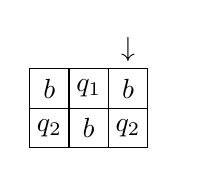
\begin{tikzpicture}
            \draw (0, 0) -- (0, 1) -- (1.5, 1) -- (1.5, 0) -- (0, 0);
            \draw (0.5, 0) -- (0.5, 1);
            \draw (1, 0) -- (1, 1);
            \draw (0, 0.5) -- (1.5, 0.5);

            \node at (0.25, 0.25) {$q_2$};
            \node at (0.75, 0.25) {$b$};
            \node at (1.25, 0.25) {$q_2$};

            \node at (0.25, 0.75) {$b$};
            \node at (0.75,  0.75) {$q_1$};
            \node at (1.25, 0.75) {$b$};

            \onslide<8->{
              \node at (1.25, 1.25) {$\downarrow$};
              \node at (2, 0.5) {\xmark};
            }
          \end{tikzpicture}
        }
      \end{center}
    \end{column}
  \end{columns}
\end{frame}

\againframe<4>{abstractions}


\begin{frame}{Conclusion}
  \begin{itemize}
    \item a first fully formalised reduction from \textbf{3SAT} to \textbf{Clique}
    \item nice proofs hard to obtain
  \end{itemize}

  \vspace{5ex}

  Roadmap:
  \begin{itemize}
    \item work out the details of Cook's Theorem
    \item tools for SAT-programming/ intermediate problems
    \item a formalisation of Cook's Theorem
    \item \ldots 
  \end{itemize}
\end{frame}

\miniframesoff
\section{}

\begin{frame}{LOC}
  \begin{center}
  \begin{tabular}{cccc}
    \multicolumn{2}{c}{Component} & Spec & Proof \\
    \midrule
    \multicolumn{2}{c}{Basic definitions\footnote{due to F. Kunze}} & 271 & 619\\
    \multicolumn{2}{c}{Preliminaries} & 118 & 297 \\
    \multicolumn{2}{c}{Higher-order RT} & 64 & 182 \\
    \midrule
    \multirow{2}{*}{SAT} & Main & 69 & 225 \\
    & RT & 75 & 227 \\
    \midrule
    \multicolumn{2}{c}{$k$-SAT} & 24 & 70 \\
    \midrule
    \multirow{2}{*}{Clique} & Main & 59 & 152 \\
    & RT & 30 & 112 \\
    \midrule
    \multirow{2}{*}{3-SAT to Clique} & Main & 264 & 667 \\
    & RT & 41 & 199\\
    \midrule
    \multicolumn{2}{c}{Total} & 1015 & 2750

  \end{tabular}
  \end{center}
\end{frame}

\begin{frame}{Representation of SAT}

\begin{align*}
  x : \var := \nat&& 
  L : \literal := \bool \times \var \\
  C : \clause := \listsof \literal &&
  N : \cnf := \listsof \clause 
\end{align*}
\begin{align*}
  \color{gray}(x_0 \lor \overline{x_1} \lor x_2) &\color{gray}\land (x_0 \lor x_3 \lor x_1)\\
  [[(\btrue, 0), (\bfalse, 1), (\btrue, 2)]&, [(\btrue, 0), (\btrue, 3), (\btrue, 1)]]
\end{align*}

\[ a : \assgn := \listsof \bool\]
\begin{align*}   
  {\color{gray}\{x_0 \mapsto \btrue, x_1 \mapsto \bfalse, x_2 \mapsto \bfalse, x_3 \mapsto \bfalse\}}\qquad 
  [\btrue, \bfalse, \bfalse, \bfalse] 
\end{align*}
\end{frame}

\begin{frame}{The Reduction Relation}
  \TODO
\end{frame}

\begin{frame}{The Reduction Function}
  \TODO
\end{frame}

\begin{frame}[allowframebreaks]{References}
  \nocite{Sipser:TheoryofComputation}
  \bibliographystyle{apalike}
  \bibliography{references}{}
\end{frame}
\end{document}
